\documentclass[a4paper]{article}

%Moduli utilizzati
\usepackage[italian]{babel}
\usepackage[utf8]{inputenc}
\usepackage{titling}
\usepackage{graphicx}
\usepackage{float}
\usepackage[nottoc]{tocbibind}
\usepackage{tabularx}
\usepackage{longtable}
\usepackage{hyperref}  
\usepackage{xspace}

%Setup
\hypersetup{
    colorlinks,
    citecolor=black,
    filecolor=black,
    linkcolor=black,
    urlcolor=black
}

%Nuovi comandi
\newcommand{\subtitle}[1]{%
  \posttitle{%
    \par\end{center}
    \begin{center}\large#1\end{center}
    \vskip0.5em}%
}

\newcommand{\net}{Ne-t\xspace}
\newcommand{\mytitle}{PadovaCard}
\newcommand{\mydegree}{Tesi di Laurea Triennale}
\newcommand{\glossario}[1]{\textit{#1\ped{\ped{G}}}}
%\newcommand{\glossario}[1]{#1}
\newcommand{\definizione}[1] {\textbf{#1}:}
\newcommand{\vivaticket}{VivaTicket\xspace}
\newcommand{\tlite}{Tlite\xspace}
\newcommand{\charta}{Charta\xspace}
\newcommand{\cappella}{Cappella degli Scrovegni\xspace}


\pagestyle{myheadings}
\markright{Nicolò Tresoldi - PadovaCard}

\title{PadovaCard}
\subtitle{Attività di stage esterno}
\author{Nicolò Tresoldi}


%Inizio Documento
\begin{document}

%\begin{titlepage}

\begin{center}

\begin{LARGE}
\textbf{Università degli Studi di Padova}\\
\end{LARGE}

\vspace{10pt}

\begin{Large}
\textsc{Dipartimento di Matematica}\\
\end{Large}

\vspace{10pt}

\begin{large}
\textsc{Corso di laurea in Informatica}\\
\end{large}

\vspace{30pt}
\begin{figure}[htbp]
\begin{center}

\includegraphics[height=6cm]{images/logo-unipd.png}
\end{center}
\end{figure}
\vspace{30pt} 

\begin{LARGE}
\begin{center}
\textbf{\mytitle}\\
\end{center}
\end{LARGE}

\vspace{10pt} 

\begin{large}
\textsl{\mydegree}\\
\end{large}

\vspace{40pt} 

\begin{large}
\begin{flushleft}
\textit{Relatore}\\ 
\vspace{5pt} 
Prof. Mauro Conti
\end{flushleft}

\vspace{0pt} 

\begin{flushright}
\textit{Laureando}\\ 
\vspace{5pt} 
Nicolò Tresoldi
\end{flushright}
\end{large}

\vspace{40pt}

\line(1, 0){338} \\
\begin{normalsize}
\textsc{Anno Accademico 2014/2015}
\end{normalsize}

\end{center}
\end{titlepage} 
%% !TEX encoding = UTF-8
% !TEX TS-program = pdflatex
% !TEX root = ../tesi.tex
% !TEX spellcheck = it-IT

%**************************************************************
% Colophon
%**************************************************************
\clearpage
\phantomsection
\thispagestyle{empty}

\hfill

\vfill

\noindent Nicolò Tresoldi: \textit{\mytitle,}
\mydegree,
\textcopyright\ Marzo 2015.
\maketitle

\tableofcontents

\listoftables

\listoffigures

\newpage

%Capitoli

\section{Introduzione}

\subsection{PadovaCard ora}
PadovaCard è un pacchetto ideato per chi desidera visitare la città. 
I punti di forza sono:
\begin{itemize}
\item Utilizzo gratuito dei mezzi di trasporto pubblici comunali;
\item Parcheggio gratuito in alcune zone;
\item Noleggio di veicoli, biciclette, segway a prezzo scontato;
\item Accesso gratuito alle strutture convenzionate.
\end{itemize}
\`E acquistabile con validità di 48 e 72 ore, contate dal momento in cui la PadovaCard viene ritirata allo sportello informazioni assistenza turistica (\glossario{IAT}).
La carta si presenta come in figura \ref{immaginePadovaCard}, e non presenta nessun tipo di circuito, banda magnetica o codice stampato. 
Proprio per questo motivo, nonostante sia una tessera personale e non cedibile, non c'è modo di verificare chi ne è l'intestatario.\\

\begin{figure}[H]
\centering
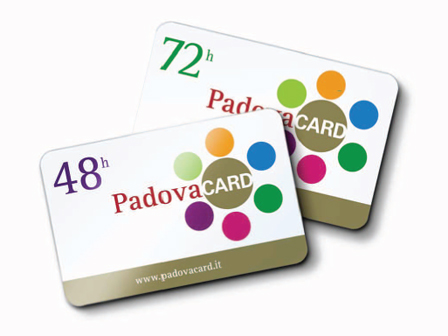
\includegraphics[width=0.6\textwidth]{images/padovacard.jpg}
\caption{Veste grafica dell'attuale PadovaCard}\label{immaginePadovaCard}
\end{figure}

Per acquistare una PadovaCard l'\glossario{utente} può recarsi ad uno degli sportelli IAT che si trovano sul territorio della città di Padova o in uno dei punti vendita autorizzati (hotel, tabaccherie, etc.).\\

\label{cappella}
La \cappella è uno tra i luoghi d'interesse più visitati, ed è convenzionato con PadovaCard. La visita alla cappella presenta un ingresso contingentato, ovvero il numero di visitatori per ogni visita è fissato, e per questo è necessario prenotare la propria visita, definendo data e fascia oraria. Non è possibile visitare la \cappella senza prenotazione. \\

Questo vincolo fa si che chiunque acquisti una PadovaCard con l'intenzione di visitare la \cappella è obbligato a prenotarne la visita. Questo è possibile farlo se si acquista la PadovaCard in un punto vendita autorizzato, oppure attraverso la piattaforma \vivaticket.
\`E inoltre attivo un call center che permette agli utenti di acquistare una PadovaCard collegata ad un ingresso in \cappella.
In questi ultimi due casi la PadovaCard verrà poi ritirata presso un punto vendita o direttamente alla \cappella.\\

I principali problemi di funzionamento dell'attuale PadovaCard sono:
\begin{itemize}
\item La PadovaCard non è nominativa;
\item Il sistema non è informatizzato e non prevede alcun tipo di tracciamento;
\item L'utente è obbligato in tutti i casi a passare da uno IAT per il ritiro della PadovaCard;
\item La piattaforma di vendita è frammentata e non comunica pienamente le offerte della PadovaCard;
\item Il sistema di vendita è frammentato tra OSS e \tlite.
\end{itemize}

La nuova PadovaCard si pone l'obbiettivo di risolvere questi problemi.



\subsection{OSS}\label{oss}
\subsubsection{Overview}
\glossario{OSS} è una piattaforma sviluppata da \net per la gestione del call center e degli sportelli \glossario{IAT} e dei relativi operatori.
Gli operatori si autenticano su questo software per gestire la vendita dell'attuale PadovaCard\footnote{Sia OSS che \tlite possono vendere la PadovaCard, salvando i dati relativi alla vendita in due diverse basi di dati. SI tratta di un problema dell'attuale sistema.} e di ogni altra merce in vendita agli sportelli \glossario{IAT}. 
OSS permette agli operatori di visualizzare il rendiconto delle vendite e al personale operatvio di compiere interrogazioni sulla base di dati.

\subsubsection{Dettagli tecnici}
Il software è scritto in \glossario{Cake Php} e si basa sull'architettura \glossario{MVC}. Come previsto da MVC sono presenti dei model, uno per ogni tabella del database, tali model si occupano di comunicare col database e di manipolare e verificare i dati che vengono estratti ed inseriti.
Per ogni model è presente un controller, che fornisce la logica al sistema attraverso vari metodi. Ad ogni controller sono collegate più view, ovvero le interfaccie utente. Una view è una pagina con cui l'utente interagisce e ogni view deve essere associata ad un controller di cui chiamerà i metodi.\\

Il database su cui si basa il sistema è un database \glossario{MySql}.

\subsection{\tlite}
\tlite è il software sviluppato da \charta che si trova dietro la piattaforma \vivaticket, e che gli operatori utilizzano per gestire la vendita delle PadovaCard\footnote{Vedi nota 1.} con annessa prenotazione alla \cappella.
Non trattandosi di un software sviluppato da \net si è dovuto adattare i requisiti ai limiti imposti da tale software.
Il limite principale è la mancanza di comunicazione tra \tlite e il software sviluppato causato da una mancanza di \glossario{API} pubbliche di \tlite.\\

Si sono comunque rivelate necessarie alcune modifiche minori al software e per questo è stato svolto un incontro tra gli sviluppaotri di \tlite e quelli di \net.
Ai fini di questo documento non è necessario conoscere il funzionamento di \tlite nel suo insieme, mentre i punti d'interesse per la progettazione del nuovo sistema per PadovaCard saranno presentati nella sezione \ref{progettazione}.

\subsection{Lavoro svolto}
Il focus dello stage è stato sui seguenti punti:
\begin{itemize}
\item Analizzare i requisiti del sistema PadovaCard, il risultato è visibile alla Sezione \ref{analisideirequisiti};
\end{itemize}

\subsubsection{Analisi dei requisiti}
Di seguito viene descritto l'approccio seguito per generare una dettagliata analisi dei requisiti, il cui risultato è presentato nella Sezione \ref{analisideirequisiti}.
L'azienda \net ha fornito al tirocinante un documento in cui vengono descritti gli obbiettivi e le criticità del nuovo sistema per la Padovacard. Dallo studio di tale documento il tirocinante ha potuto definire il piano di lavoro dello stage.\\

L'analisi degli obbiettivi e del funzionamento del sistema ad alto livello è stato poi discusso in diverse riunioni tra i membri del team di sviluppo, ponendo un focus particolare sulle difficoltà inerenti alla \cappella, esposte nella Sezione \ref{cappella}.\\

Da queste riunioni il tirocinante ha estratto i dettagli funzionali dell’applicazione.
Per esprimere in modo chiaro i requisiti individuati si è ricorso al formalismo UML - Casi d'uso, anch'essi visionabili alla Sezione \ref{analisideirequisiti}.\\

L'individuazione dei requisiti è stata fatta corretamente già alla prima iterazione, mentre i casi d'uso e la loro descrizione dettagliata sono stati modificati più volte, al fine di eliminare ogni possibile ambiguità.
\subsection{Risultati a fine stage}
\section{Studio di fattibilità delle possibili soluzioni}
Per poter comprendere le soluzioni di seguito proposte è necessario conoscere il software \glossario{OSS}, presentato alla Sezione \ref{oss}.
La seguente immagine presenta il funzionamento del nuovo sistema PadovaCard nel suo complesso.
Per maggiori dettagli vedere l'analisi dei requisiti alla Sezione \ref{analisideirequisiti}.
\begin{figure}[H]
\centering
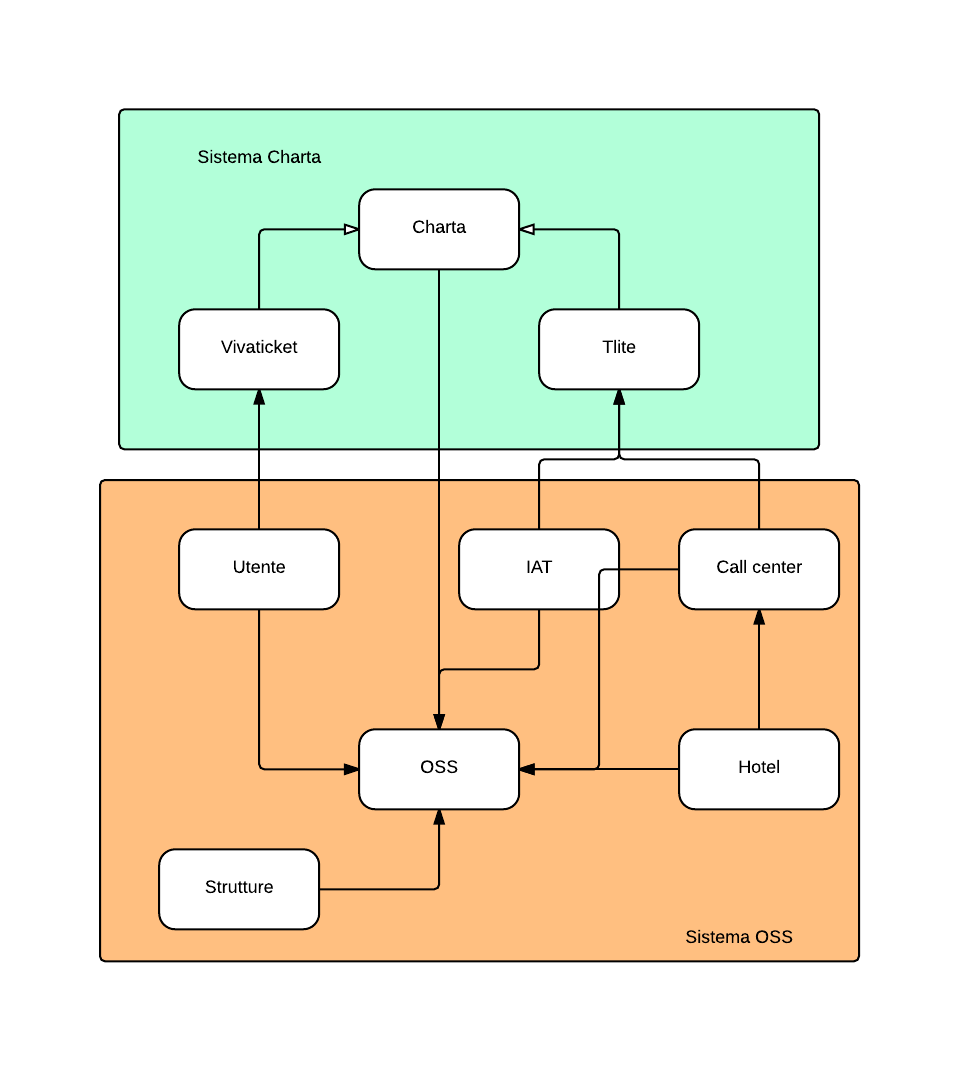
\includegraphics[width=0.9\textwidth]{images/Schema_introduttivo.png}
\caption{Architettura di alto livello di OSS}
\end{figure}

\subsection{Espansione del sistema OSS}
Per questa soluzione non è prevista la produzione di un sistema ex-novo, ma un ampliamento del sistema \glossario{OSS} già esistente affinchè soddisfi i requisiti richiesti.
\begin{figure}[H]
\centering
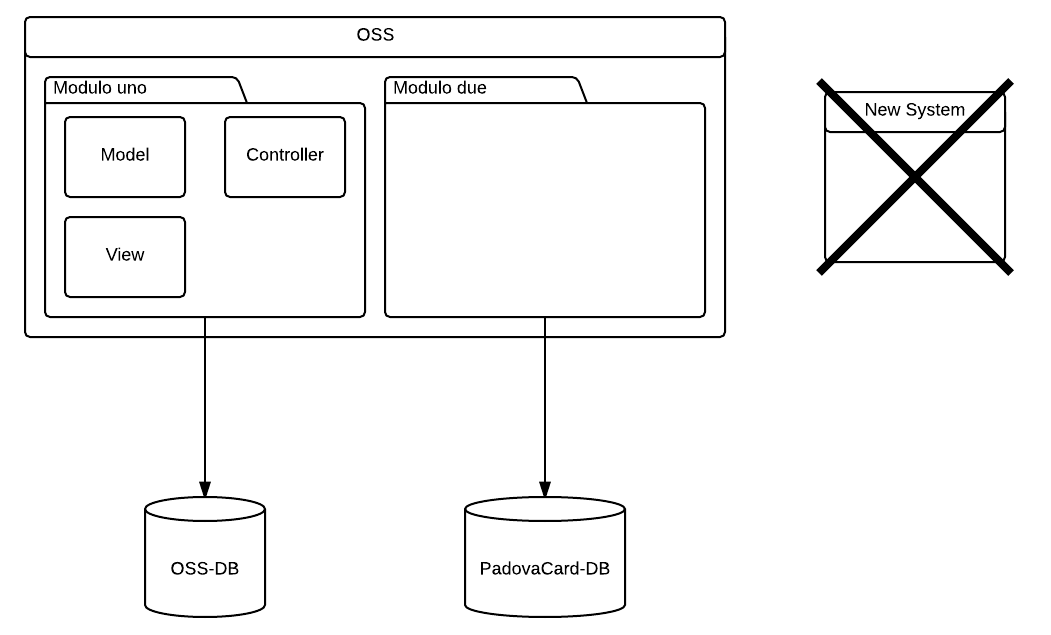
\includegraphics[width=0.7\textwidth]{images/Espansione_del_sistema_OSS.png}
\caption{Diagramma della soluzione: Espansione del sistema OSS}
\end{figure}
Nella figura tutti i componenti interni al modulo uno sono quelli già esistenti che non andranno modificati.
I componenti all'interno del modulo due sono quelli che verranno progettati e sviluppati per soddisfare i requisiti annessi alla nuova PadovaCard.\\

Il database \glossario{OSS} è quello già presente mentre il database PadovaCard è quello che andrà creato. In alternativa si può utilizzare un unico database e creare nuove tabelle per la gestione della PadovaCard.
Questa soluzione soddisfa il requisito di avere un unica piattaforma per gestire tutto, dalla vendita della PadovaCard, alla vendita di altri articoli, alla gestione dei pagamenti e degli operatori.\\

Uno svantaggio è che il tirocinante, se pur a conoscenza del linguaggio PHP e dell'architettura MVC, non ha mai sviluppato con CakePHP, inoltre dovrebbe studiare il funzionamento del sistema esistente nel dettaglio. Tale studio può limitarsi alle sezioni del software di interesse, ma si prevede un costo di apprendimento iniziale elevato.\\
\textbf{Vantaggi:}
\begin{itemize}
\item Non viene creato un nuovo sistema;
\item Necessaria meno documentazione;
\item Il pagamento di PadovaCard e altri articoli è unico;
\item I dati relativi alla PadovaCard sono logicamente separati, mentre quelli amministrativi sono accorpati.
\end{itemize}
\textbf{Svantaggi:}
\begin{itemize}
\item Necessario l'apprendimento del funzionamento di OSS;
\item Necessario l'apprendimento del funzionamento di CakePHP;
\item Rischio di introdurre errori in un sistema funzionante;
\end{itemize}

\subsection{Nuovo sistema per gli acquisti}
In questa soluzione si prevede di progettare e realizzare un nuovo sistema che si occuperà della vendita delle PadovaCard e degli altri articoli. Il sistema OSS resterà presente in parallelo per la gestione delle rimanenti necessità.

\begin{figure}[H]
\centering
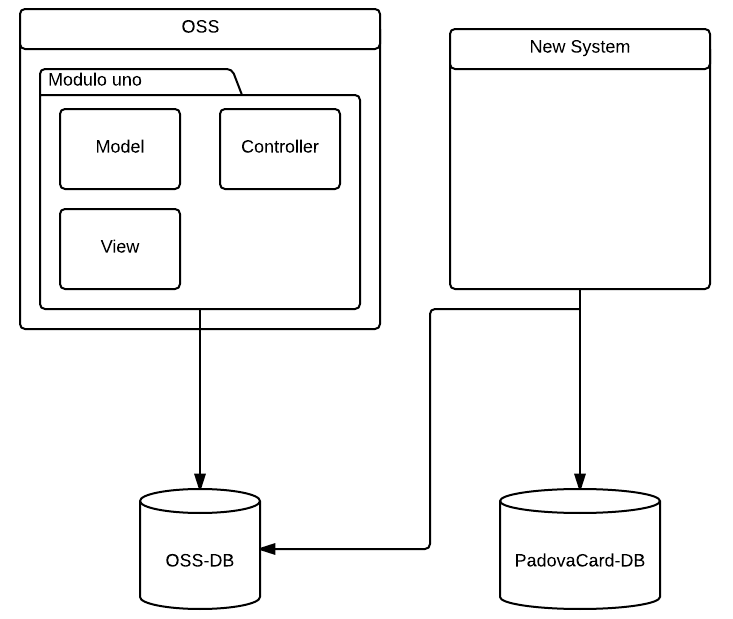
\includegraphics[width=0.7\textwidth]{images/Nuovo_sistema_per_gli_acquisti.png}
\caption{Diagramma della soluzione: Nuovo sistema per gli acquisti}
\end{figure}
A differenza della soluzione precedente in questo caso il sistema OSS ora esistente non viene modificato, e si crea un nuovo sistema, identificato in figura come come new System. Tale sistema non interagisce in alcun modo con il sistema OSS, ma comunica invece con il database OSS per la scrittura degli acquisti, mentre comunicherà con il database PadovaCard per tutti i dettagli riguardanti le sole PadovaCard.\\

Tale soluzione presenta il vantaggio per il tirocinante di non dover apprendere CakePHP e il funzionamento di OSS, ma c'è il rischio di una frammentazione dei dati. \\
\textbf{Vantaggi:}
\begin{itemize}
\item Nuovo sistema, separato ed indipendente per la vendita della PadovaCard;
\item Il sistema OSS non viene modificato;
\item Il pagamento di PadovaCard e altri articoli è unico;
\item I dati relativi alla PadovaCard sono logicamente separati, mentre quelli amministrativi sono accorpati.
\end{itemize}
\textbf{Svantaggi:}
\begin{itemize}
\item Necessaria la progettazione di un nuovo sistema;
\item Il codice sorgente relativo a vendita e pagamento verrebbe duplicato;
\item Necessaria una maggiore documentazione;
\item Si hanno due sistemi che in parte fanno la stessa cosa.
\end{itemize}

\subsection{Sistema ibrido}
Si tratta di una soluzione che ibrida le due appena viste. In questo caso viene creato un nuovo sistema, che si occuperà della sola vendita della PadovaCard (ed eventualmente dei singoli accessi ai luoghi d'interesse), mentre OSS continuerà a vendere tutti gli altri articoli. 
I due sistemi comunicheranno tra loro e l'operatore potrà passare da uno all'altro in modo automatico in base a cosa desidera vendere. \\

Il pagamento finale sarà possibile su entrambe le piattaforme e comprenderà gli articoli venduti su entrambe.

\begin{figure}[H]
\centering
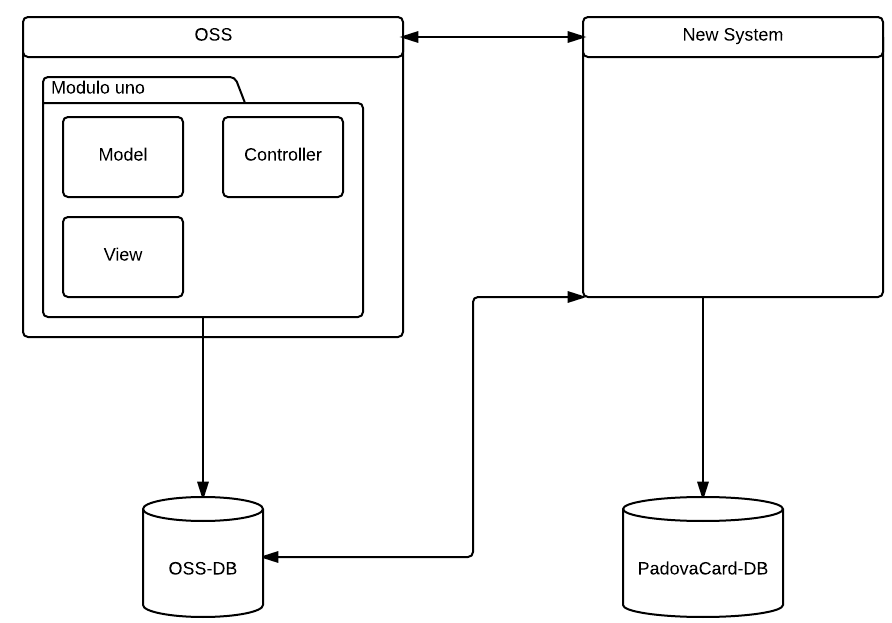
\includegraphics[width=0.7\textwidth]{images/Sistema_ibrido.png}
\caption{Diagramma della soluzione: Sistema ibrido}
\end{figure}
Questa soluzione prevede che il sistema OSS non venga modificato se non per il redirect al nuovo sistema e la conferma al nuovo sistema dell'avvenuto pagamento. 
Nel database OSS saranno salvati i record di vendita, comprese le PadovaCard, ma tutti i dettagli relativi ad esse saranno separati nel database PadovaCard (o in un'altra tabella nello stesso database). \\
\textbf{Vantaggi:}
\begin{itemize}
\item Nuovo sistema, separato ed indipendente per la vendita della PadovaCard;
\item Il sistema OSS viene modificato solo in superficie, con un costo basso;
\item Per l'operatore il pagamento di PadovaCard e altri articoli è unico;
\item I dati relativi alla PadovaCard sono logicamente separati, mentre quelli amministrativi sono accorpati.
\end{itemize}
\textbf{Svantaggi:}
\begin{itemize}
\item Necessaria la progettazione di un nuovo sistema;
\item L'operatore passando da un sistema all'altro si troverebbe una diversa interfaccia;
\item Necessaria una maggiore documentazione;
\end{itemize}

\subsection{Conclusioni}
La soluzione due, Nuovo sistema per gli acquisti, presenta maggiori svantaggi rispetto ai vantaggi, e per questo è stata immediatamente scartata. \\

Le soluzioni uno e tre hanno molti vantaggi in comune, come la separazione logica dei dati relativi alla PadovaCard e l'unificazione del sistema di pagamento, ma ritengo che la soluzione uno presenti un minor costo di sviluppo in termini di uomo/ora, e sia quindi da preferire.  
\clearpage\null\newpage
\section{Analisi dei requisiti}\label{analisideirequisiti}
\subsection{Casi d'uso}

I casi d'uso sono presentati con la notazione \glossario{UML}.
Ad ogni caso d'uso è associato un titolo ed un codice che segue il seguente formalismo:

\begin{center}
\textbf{UC[F]\{Gerarchia\}}
\end{center}

Dove:
\begin{itemize}
\item UC sono i casi d'uso obbligatori;
\item UCF sono i casi d'uso facoltativi;
\item Gerarchia identifica la relazione gerarchica che c'è tra i requisiti di uno stesso tipo. C'è quindi una struttura gerarchica per ogni tipologia di requisito.
\end{itemize}

\subsubsection{Caso d'uso UC: Operazioni ad alto livello}\label{UC}
Il seguente diagramma presenta una visione di alto livello dei casi d'uso obbligatori. Ogni caso d'uso verrà poi analizzato nel dettaglio nelle sezioni successive. I casi d'uso opzionali si trovano dalla Sezione \ref{UCF} in poi.

\begin{figure}[H]
\centering
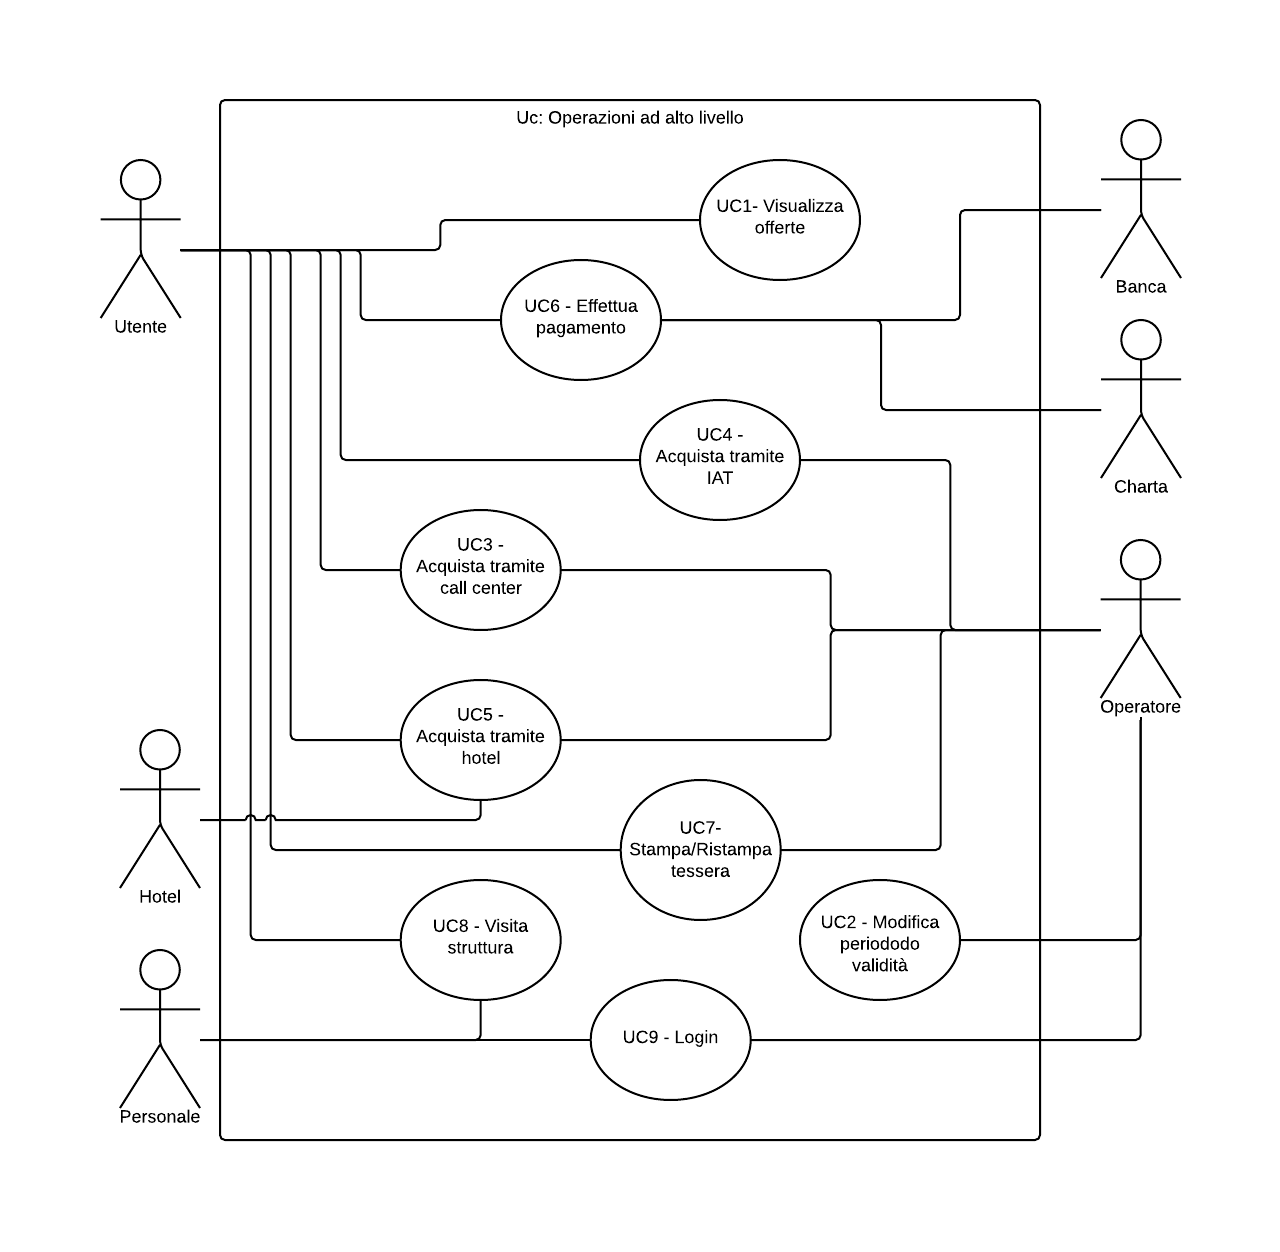
\includegraphics[width=1\textwidth]{images/UC.png}
\caption{Caso d'uso UC: Operazioni ad alto livello}
\end{figure}

\subsubsection{Caso d'uso UC1: Consultazione offerte}\label{UC1}
\begin{figure}[H]
\centering
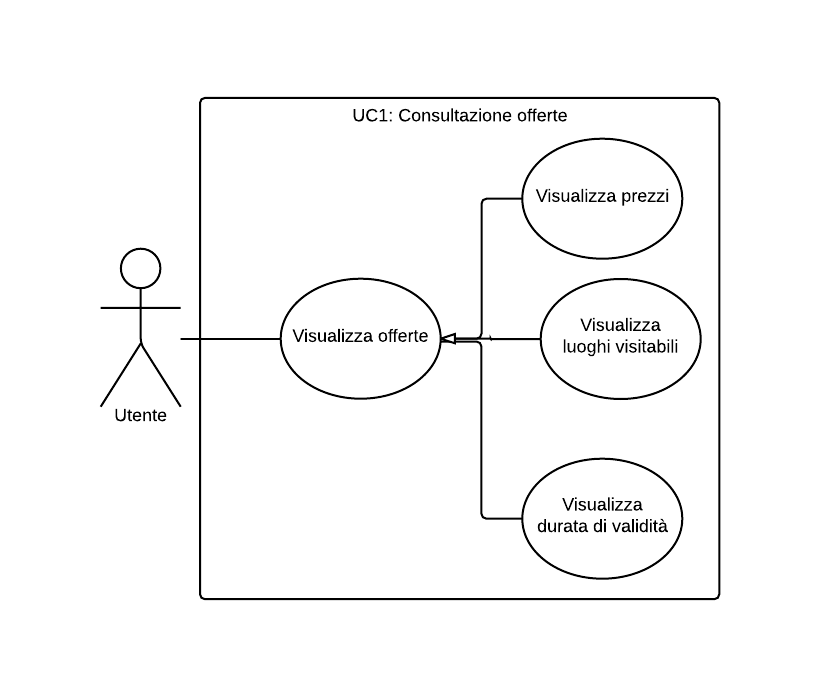
\includegraphics[width=1\textwidth]{images/UC1.png}
\caption{Caso d'uso UC1: Consultazione offerte}
\end{figure}
\begin{itemize}
\item \textbf{Attori:} Utente;
\item \textbf{Descrizione:} L'utente deve poter consultare online le offerte relative alla propria PadovaCard. Tali offerte comprendono i vari pacchetti con cui la PadovaCard viene proposta, i luoghi con essa visitabili ed i relativi costi e periodo di validità. Si tratta di un portale statico;

\item \textbf{Flusso principale degli eventi:}
	\begin{itemize}
		\item L'utente si collega al portale tramite browser;
		\item L'utente visualizza le informszioni a cui è interessato.
	\end{itemize}
\end{itemize}

\subsubsection{Caso d'uso UC2: Modifica periodo validità}
\begin{figure}[H]
\centering
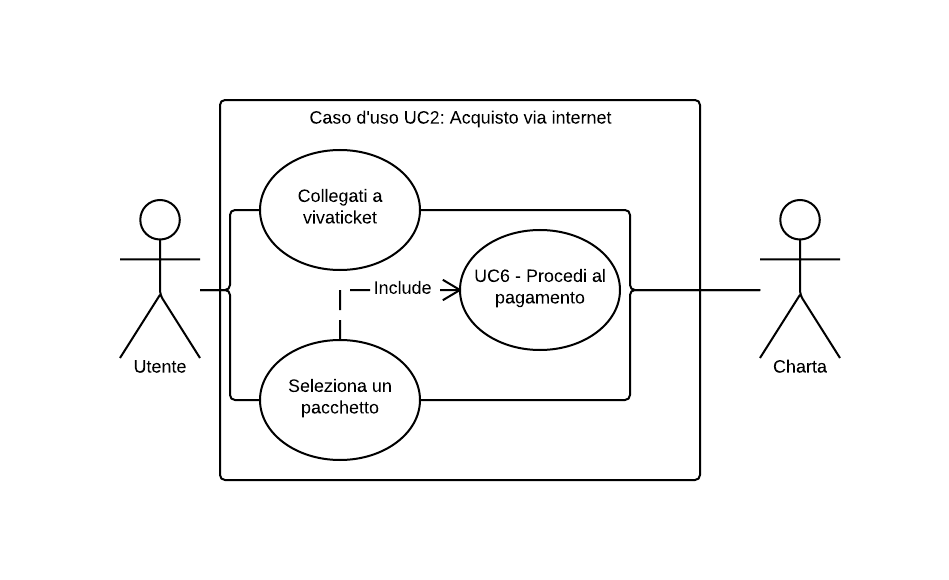
\includegraphics[width=1\textwidth]{images/UC2.png}
\caption{Caso d'uso UC2: Modifica periodo validità}
\end{figure}
\begin{itemize}
\item \textbf{Attori:} Utente, operatore;
\item \textbf{Descrizione:} L'utente ha acquistato una o più PadovaCard, e nel momento dell'acquisto ha definito il loro periodo di validità, selezionando data e ora, come descritto in UC6, alla Sezione \ref{UC6}. L'utente decide però di modificare tale periodo di validità, non gli è consentito farlo da solo, dovrà quindi contattare un operatore, call center o IAT e far modificare il peridoo di validità, con il vincolo che se è prevista una visita alla cappella degli Scrovegni, essa dovrà trovarsi sempre dentro l'arco temporale di validità della tessera;
\item \textbf{Precondizione:} L'utente desidera modificare il periodo di validità della PadovaCard;
\item \textbf{Postcondizione:}  Il periodo di validità della PadovaCard è modificato.
\end{itemize}


\subsubsection{Caso d'uso UC3: Acquisto via call center}\label{UC3}
\begin{figure}[H]
\centering
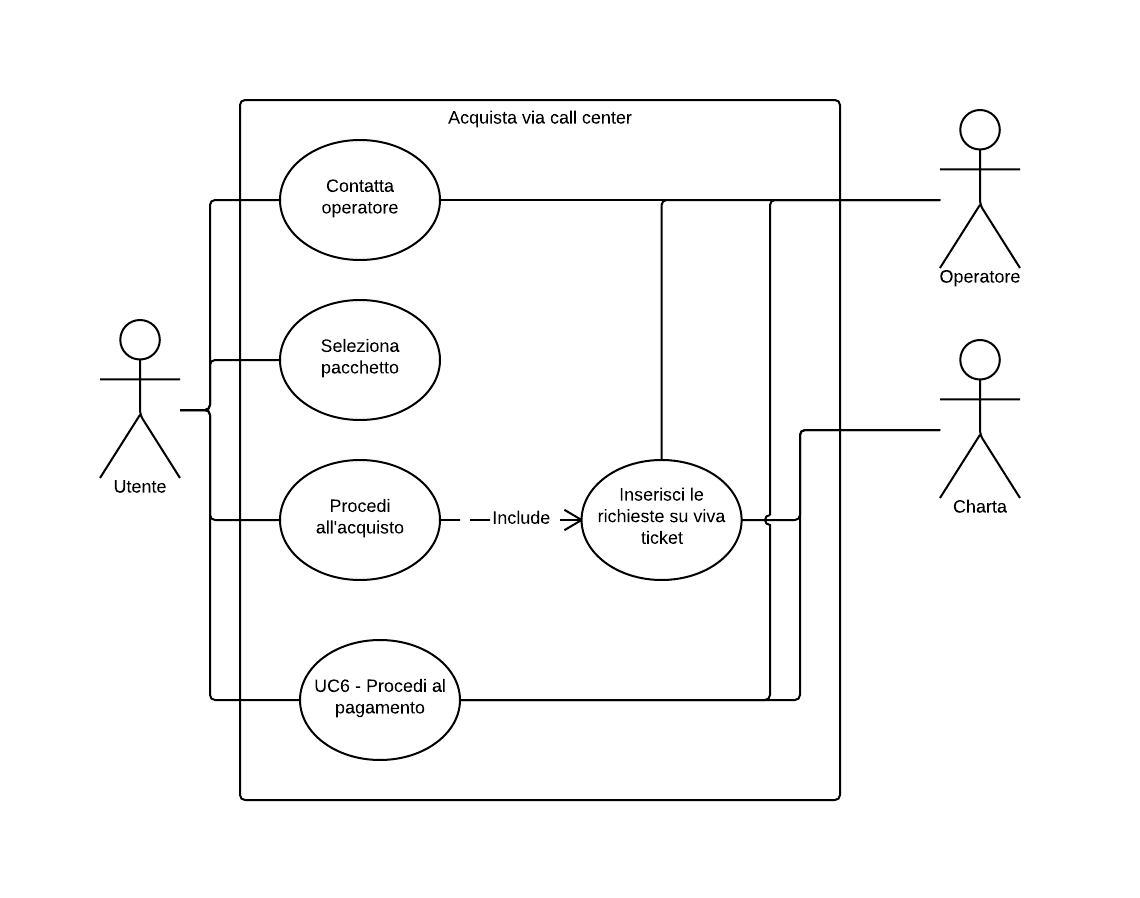
\includegraphics[width=1\textwidth]{images/UC3.png}
\caption{Caso d'uso UC3: Acquisto via call center}
\end{figure}
\begin{itemize}
\item \textbf{Attori:} Utente, operatore, \charta;
\item \textbf{Descrizione:} L'utente contatta il call center, e gli operatori guideranno l'utente nella scelta di uno dei pacchetti disponibili. Quando l'utente ha deciso l'operatore prenota su \tlite acquistando un biglietto a 0 euro. L'ultima operazione per poter ricevere le PadovaCard è il pagamento, descritto in \ref{UC6}.
\item \textbf{Precondizione:} L'utente desidera comprare una o più padova card;
\item \textbf{Flusso principale degli eventi:}
	\begin{itemize}
		\item L'utente chiama il call center;
		\item L'utente, guidato dall'operatore sceglie quale pacchetto acquistare;
        \item L'operatore procede all'eventuale prenotazione della visita alla \cappella;
        \item L'operatore, su OSS, inserisce i dati dell'utente e della PadovaCard.
	\end{itemize}
\item \textbf{Postcondizione:}L'utente deve solamente pagare per completare l'acquisto.
\end{itemize}

\subsubsection{Caso d'uso UC4: Acquisto via IAT}\label{UC4}
\begin{figure}[H]
\centering
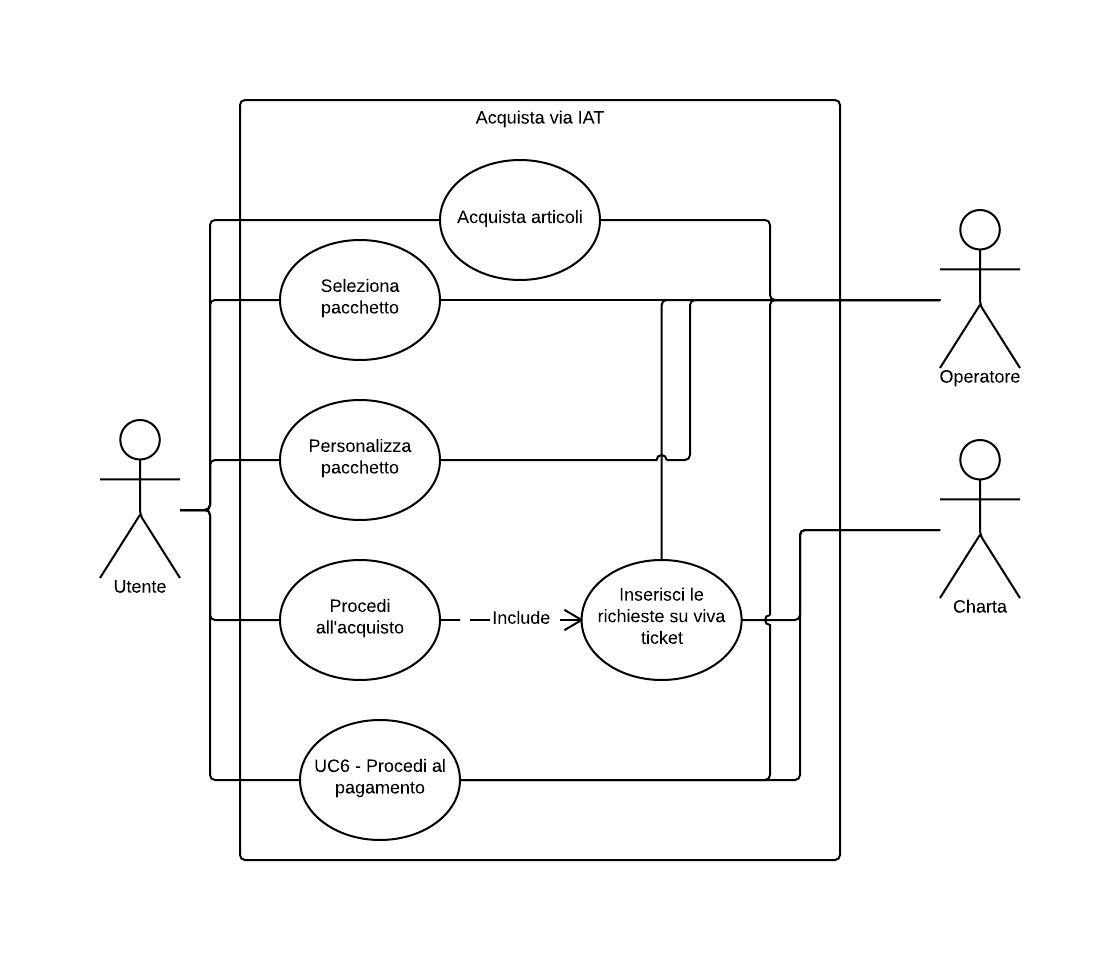
\includegraphics[width=1\textwidth]{images/UC4.png}
\caption{Caso d'uso UC4: Acquisto via IAT}
\end{figure}
\begin{itemize}
\item \textbf{Attori:} Utente, operatore, \charta;
\item \textbf{Descrizione:} L'utente si reca ad uno sportello IAT dove potrà acquistare uno degli articoli in vendita e/o una o più PadovaCard. L'operatore completerà prenota su \tlite acquistando un biglietto a 0 euro, quindi può personalizzare i pacchetti con le preferenze di visita  dell'utente. A questo punto all'utente non resta che pagare quanto acquistato con un unico pagamento, tale operazione è illustrata nella Sezione \ref{UC6}.
\item \textbf{Precondizione:} L'utente desidera comprare una o più padova card;
\item \textbf{Flusso principale degli eventi:}
	\begin{itemize}
    	\item L'utente sceglie un pacchetto;
        \item L'operatore procede alla prenotazione su \tlite;
		\item L'utente assieme all'operatore personalizza il pacchetto;
		\item L'utente può acquistare altri articoli in vendita allo IAT.
	\end{itemize}
\item \textbf{Postcondizione:}L'utente deve solamente pagare per completare l'acquisto.
\end{itemize}

\subsubsection{Caso d'uso UC5: Acquisto via hotel}\label{UCF5}
\begin{figure}[H]
\centering
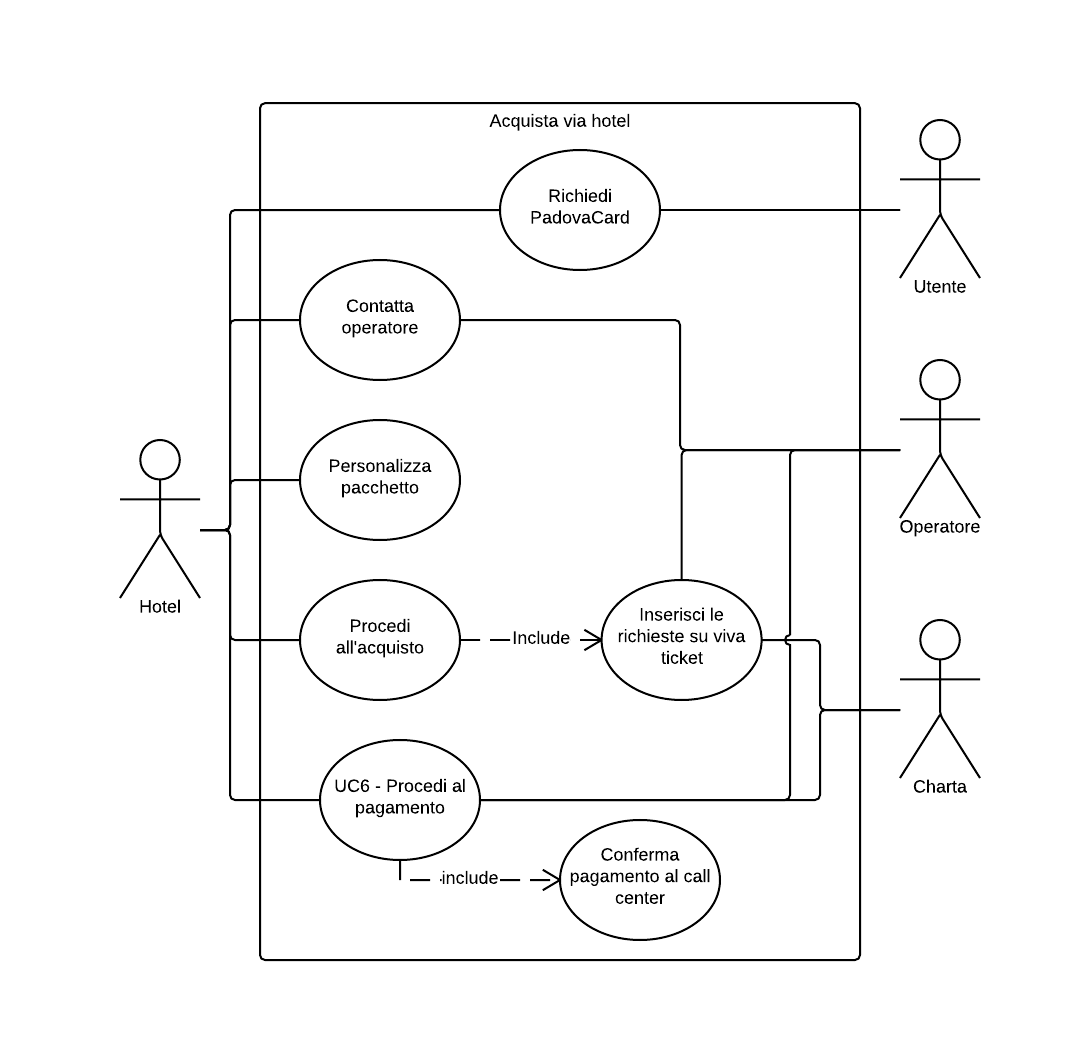
\includegraphics[width=1\textwidth]{images/UC5.png}
\caption{Caso d'uso UC5: Acquisto via hotel}
\end{figure}
\begin{itemize}
\item \textbf{Attori:} Utente, operatore, \charta, hotel;
\item \textbf{Descrizione:} L'utente riferisce ad un membro del personale dell'hotel (se quest'ultimo è convenzionato con PadovaCard) che desidera acquistare una o più PadovaCard. Il personale dell'hotel comunicherà con il call center tramite un canale a priorità maggiore di quello comune, per i dettagli vedere il caso d'uso UC3 alla Sezione \ref{UC3}. Dunque il processo è identico all'acquisto via call center se non che l'hotel fa da intermediario;
\item \textbf{Precondizione:} L'utente desidera comprare una o più padova card;
\item \textbf{Flusso principale degli eventi:}
	\begin{itemize}
    	\item L'utente riferisce all'hotel che desidera comprare una o più PadovaCard;
		\item L'hotel chiama il call center;
		\item L'hotel comunica la data di visita e quale pacchetto acquistare;
        \item L'operatore procede alla prenotazione su \tlite;
        \item Si procede al pagamento.
	\end{itemize}
\item \textbf{Postcondizione:}L'utente deve solamente pagare per completare l'acquisto;
\end{itemize}

\subsubsection{Caso d'uso UC6: Pagamento}\label{UC6}
\begin{figure}[H]
\centering
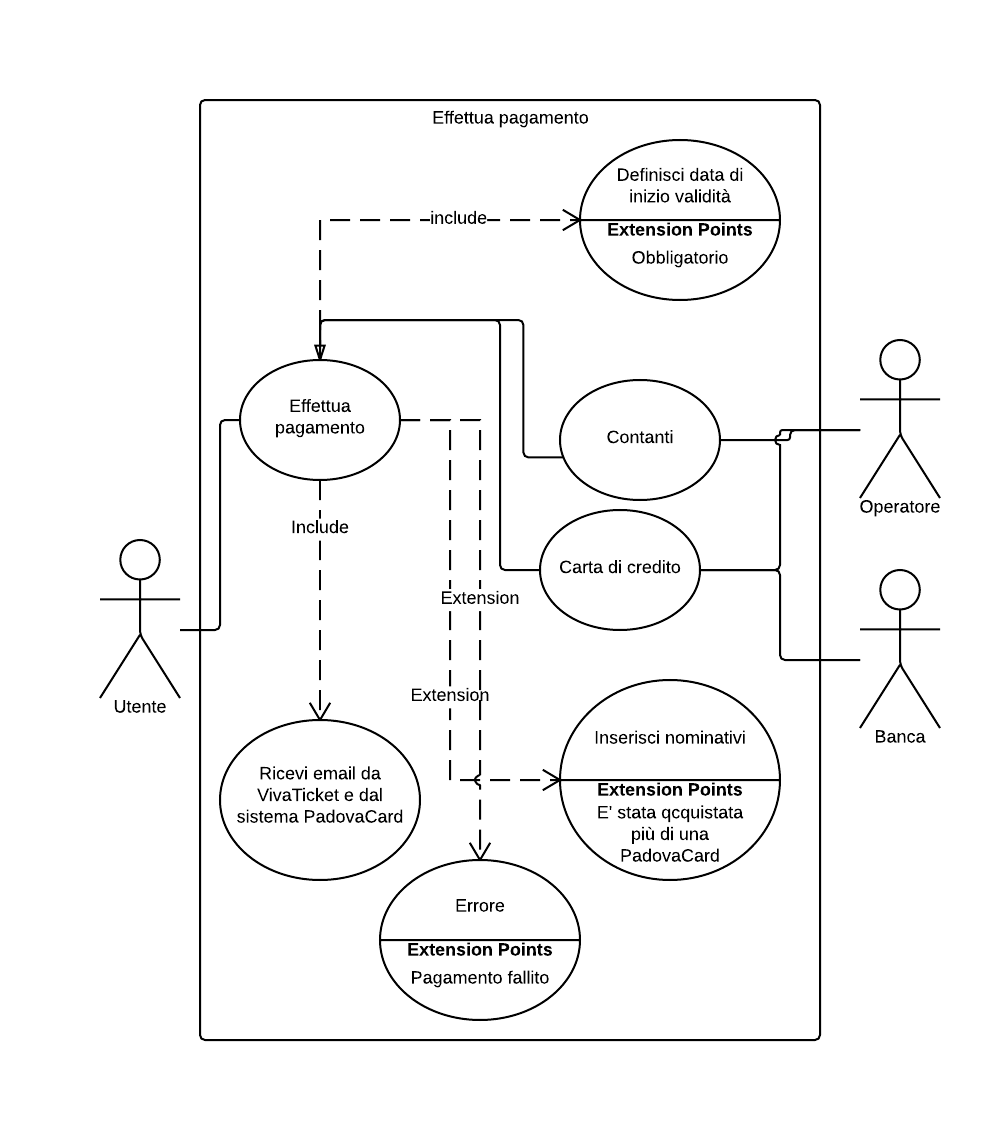
\includegraphics[width=1\textwidth]{images/UC6.png}
\caption{Caso d'uso UC6: Pagamento}
\end{figure}
\begin{itemize}
\item \textbf{Attori:} Utente, operatore, banca;
\item \textbf{Descrizione:} L'utente ha selezionato la propria PadovaCard con uno dei possibili metodi, e si appresta a pagare. E' possibile farlo sempre tramite carta di credito, mentre è possibile  in contanti solo se l'acquisto è stato fatto presso uno sportello IAT\textsuperscript{1}  e via bonifico solo dal call center. Qualora il pagamento andasse a buon fine l'utente riceverà un'unica mail dal sistema con il codice della PadovaCard e il codice di prenotazione \tlite. Qualora durante un'ordine siano acquistate più PadovaCard sarà necessario inserire un nominativo per ognuna di esse, avvalendosi di un operatore. Nel caso in cui l'acquisto avvenga via internet ciò non è possibile, ma una possibile soluzione è proposta come requisito facoltativo alla Sezione \ref{UCF3}.
Fondamentale è poi definire una data e un ora di inizio validità per la PadovaCard (la scadenza si fisserà di conseguenza), tenendo presente che se compresa, la visita alla cappella degli Scrovegni deve essere all'interno del periodo di validità.\\
\begin{footnotesize}
\textit{\textsuperscript{1} Un hotel a sua discrezione potrebbe far pagare l'utente in contanti e poi utilizzare la propria carta di credito}
\end{footnotesize}
\item \textbf{Precondizione:} L'utente ha selezionato il pacchetto da acquistare;
\item \textbf{Flusso principale degli eventi:}
	\begin{itemize}
		\item L'utente paga, via carta di credito, contanti o bonifico;
        \item L'utente stabilisce la data e l'ora di inizio del periodo di validità;
		\item L'utente riceve la mail contenente il codice della PadovaCard.
	\end{itemize}
    \item \textbf{Flusso alternativo degli eventi:}
	\begin{itemize}
    	\item Il pagamento non va a buon fine, la carta è rifiutata dalla banca o l'utente non ha abbastanza contanti;
		\item L'utente acquista più di una PadovaCard, è necessario inserire i nominativi per ognuna.
	\end{itemize}
\item \textbf{Postcondizione:} L'utente ha ricevuto la PadovaCard.
\end{itemize}

\subsubsection{Caso d'uso UC7: Stampa/ristampa tessera}
\begin{figure}[H]
\centering
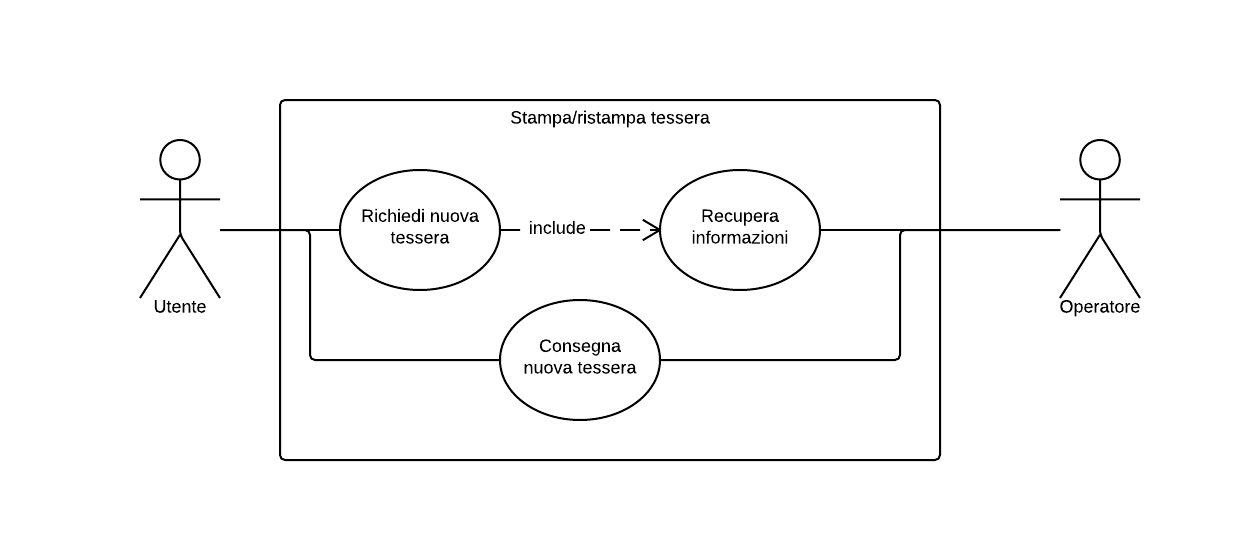
\includegraphics[width=1\textwidth]{images/UC7.png}
\caption{Caso d'uso UC7: Stampa/ristampa tessera}
\end{figure}
\begin{itemize}
\item \textbf{Attori:} Utente, operatore;
\item \textbf{Descrizione:} L'utente si reca ad uno sportello IAT e comunica la propria volontà di avere la propria PadovaCard stampata. Ricordiamo che avere la PadovaCard stampata non è strettamente necessario, in quanto è sufficiente stampare il codice ricevuto via email su carta o mostrare il codice a schermo. L'operatore recupera il codice della PadovaCard partendo dal nominativo dell'utente ed esegue la stampa;
\item \textbf{Precondizione:} L'utente desidera avere stampata la propria PadovaCard, o ha smarrito quella in suo possesso;
\item \textbf{Flusso principale degli eventi:}
	\begin{itemize}
    	\item L'utente desidera la PadovaCard stampata;
        \item L'operatore recupera il codice della PadovaCard;
        \item L'operatore stampa la PadovaCard.
    \end{itemize}
\item \textbf{Postcondizione:}  L'utente ottiene la PadovaCard stampata;
\end{itemize}

\subsubsection{Caso d'uso UC8: Visita struttura}
\begin{figure}[H]
\centering
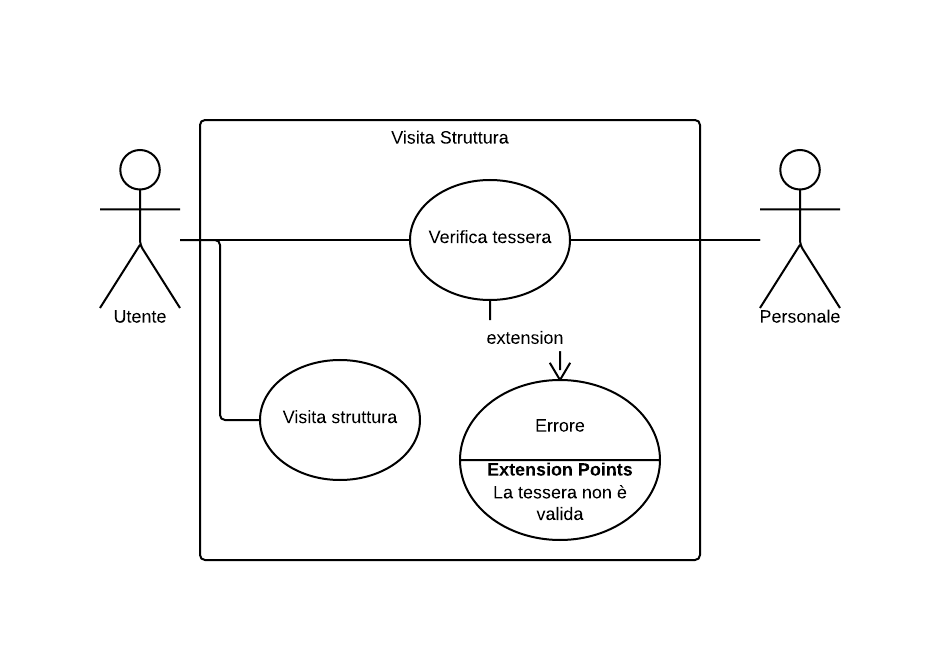
\includegraphics[width=1\textwidth]{images/UC8.png}
\caption{Caso d'uso UC8: Visita struttura}
\end{figure}
\begin{itemize}
\item \textbf{Attori:} Utente, personale;
\item \textbf{Descrizione:} Un utente munito della propria PadovaCard si reca alla struttura che desidera visitare, il personale, autenticato nel sistema legge il codice a barre (stampato o a schermo) tramite l'apposito lettore e visualizza quindi sul monitor se l'utente può visitare la struttura o meno;
\item \textbf{Precondizione:} L'utente vuole visitare una struttura, il personale è autenticato;
\item \textbf{Postcondizione:}  L'utente ha visitato la struttura;
\end{itemize}


\subsubsection{Caso d'uso UC9: Login}
\begin{figure}[H]
\centering
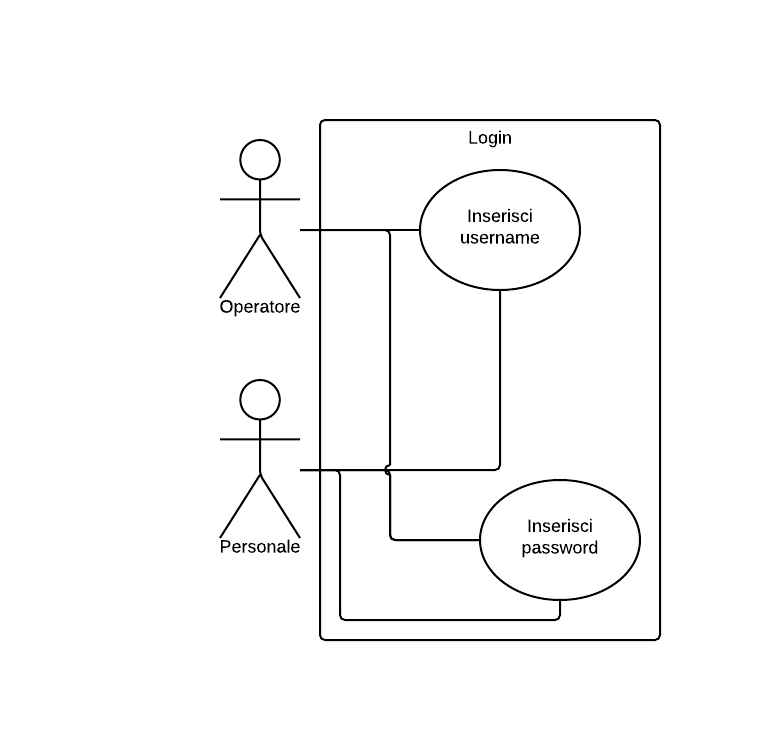
\includegraphics[width=1\textwidth]{images/UC9.png}
\caption{Caso d'uso UC9: Login}
\end{figure}
\begin{itemize}
\item \textbf{Attori:} Personale, operatore;
\item \textbf{Descrizione:} Vengono inserite le credenziali, username e password e se corretti si viene autenticati. Deve poter essere possibile recuperare e modificare la propria password;
\item \textbf{Precondizione:} Il personale e gli operatori non sono autenticati;
\item \textbf{Postcondizione:}  Il personale e gli operatori sono autenticati.
\end{itemize}

\subsubsection{Caso d'uso UCF: Operazioni ad alto livello}\label{UCF}
Il seguente diagramma mostra una visione ad alto livello dei casi d'uso facoltativi. Ogni caso d'uso è analizzato nel dettaglio nelle sezioni successive. I casi d'uso obbligatori si trovano dalla Sezione \ref{UC} in poi.
\begin{figure}[H]
\centering
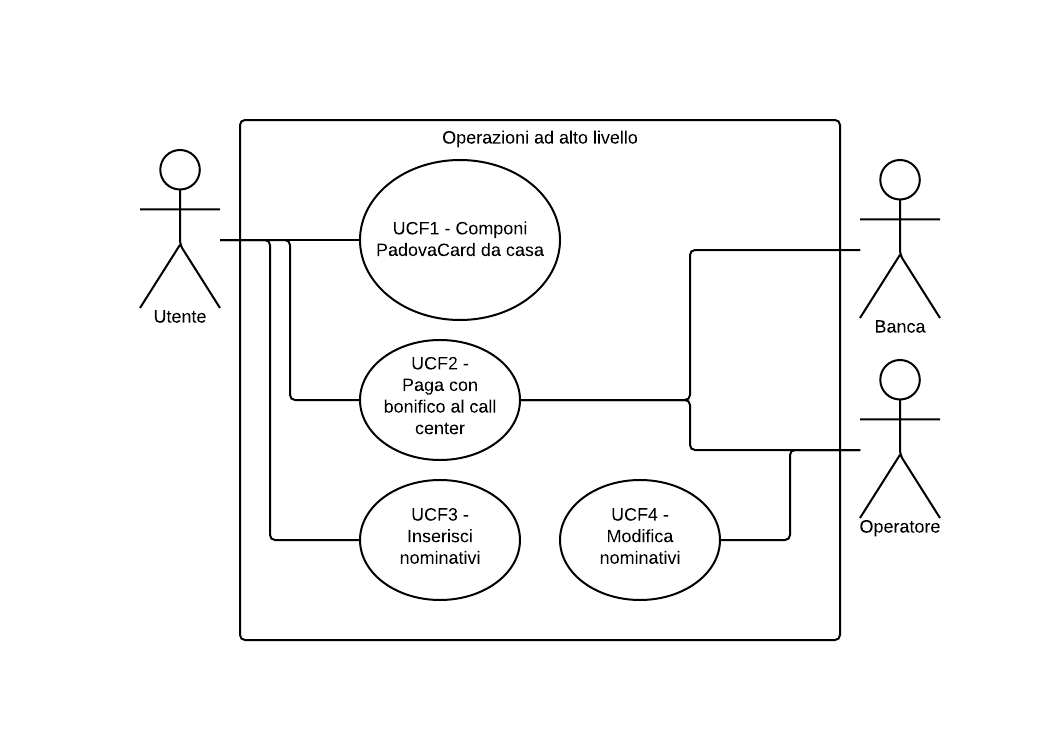
\includegraphics[width=1\textwidth]{images/UCF.png}
\caption{Caso d'uso UCF: Operazioni ad alto livello}
\end{figure}

\subsubsection{Caso d'uso UCF1: Componi PadovaCard da casa}
Questo requisito permette all'utente di personalizzare la propria PadovaCard da casa.
\begin{figure}[H]
\centering
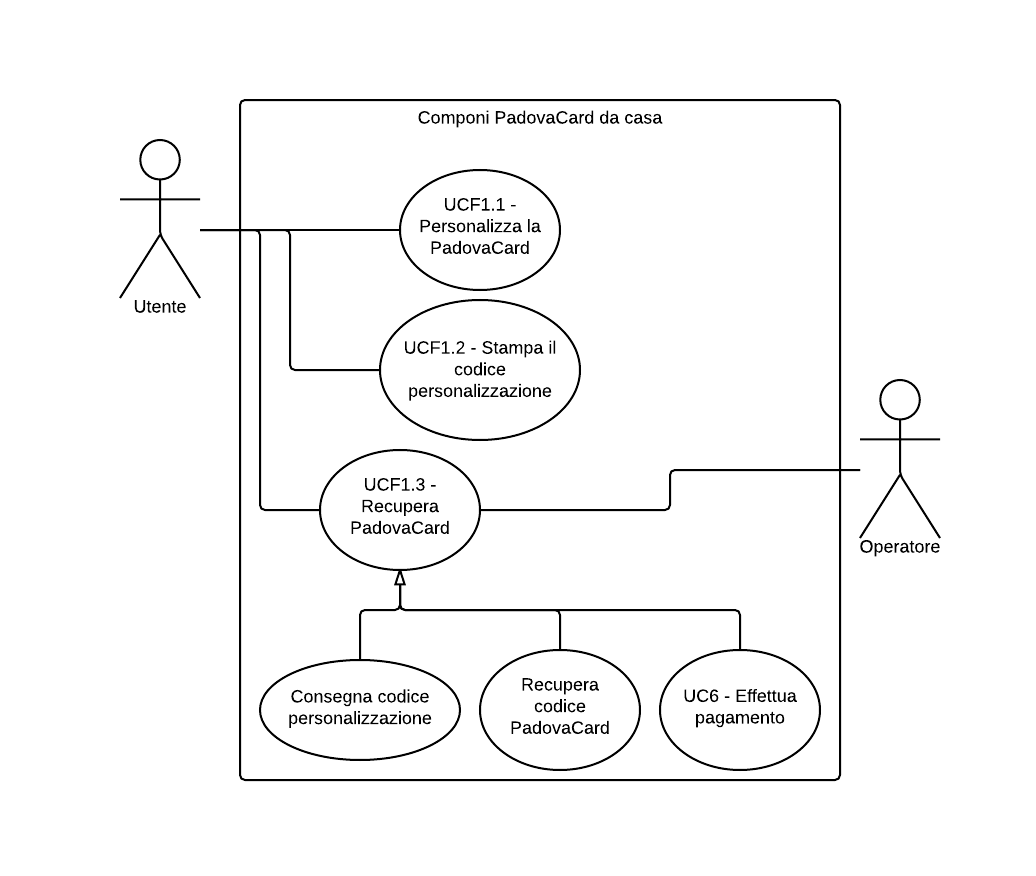
\includegraphics[width=1\textwidth]{images/UCF1.png}
\caption{Caso d'uso UCF1:  Componi PadovaCard da casa}
\end{figure}
\textbf{UCF1.1}
\begin{itemize}
\item \textbf{Attori:} Utente;
\item \textbf{Precondizione:} L'utente accede al portale;
\item \textbf{Descrizione:} L'utente tramite il portale web ha la possibilità di comporre la propria Padovacard;
\item \textbf{Postcondizione:} L'utente ha personalizzato la propria PadovaCard.
\end{itemize}

\textbf{UCF1.2}
\begin{itemize}
\item \textbf{Attori:} Utente;
\item \textbf{Precondizione:} L'utente ha personalizzato la propria PadovaCard;
\item \textbf{Descrizione:} Il portale genera un codice di personalizzazione. Tale codice non è da confondere con quello della PadovaCard, esso infatti non permette di accedere alle strutture;
\item \textbf{Postcondizione:} L'utente è in possesso di un codice di personalizzazione.
\end{itemize}

\textbf{UCF1.3}
\begin{itemize}
\item \textbf{Attori:} Utente, operatore;
\item \textbf{Precondizione:} L'utente è in possesso di un codice di personalizzazione;
\item \textbf{Descrizione:} L'utente con il proprio codice di personalizzazione si reca ad uno sportello IAT, dove l'operatore, leggendo il codice ed interrogando il sistema verrà a conoscenza di come l'utente desidera la propria PadovaCard e questo permette di velocizzarne la creazione. Da questo momento in poi il procedimento è lo stesso di UC4, visibile alla Sezione \ref{UC4}.

\item \textbf{Postcondizione:} L'utente è in possesso della PadovaCard.
\end{itemize}

\subsubsection{Caso d'uso UCF2: Acquisto via internet}
\begin{figure}[H]
\centering
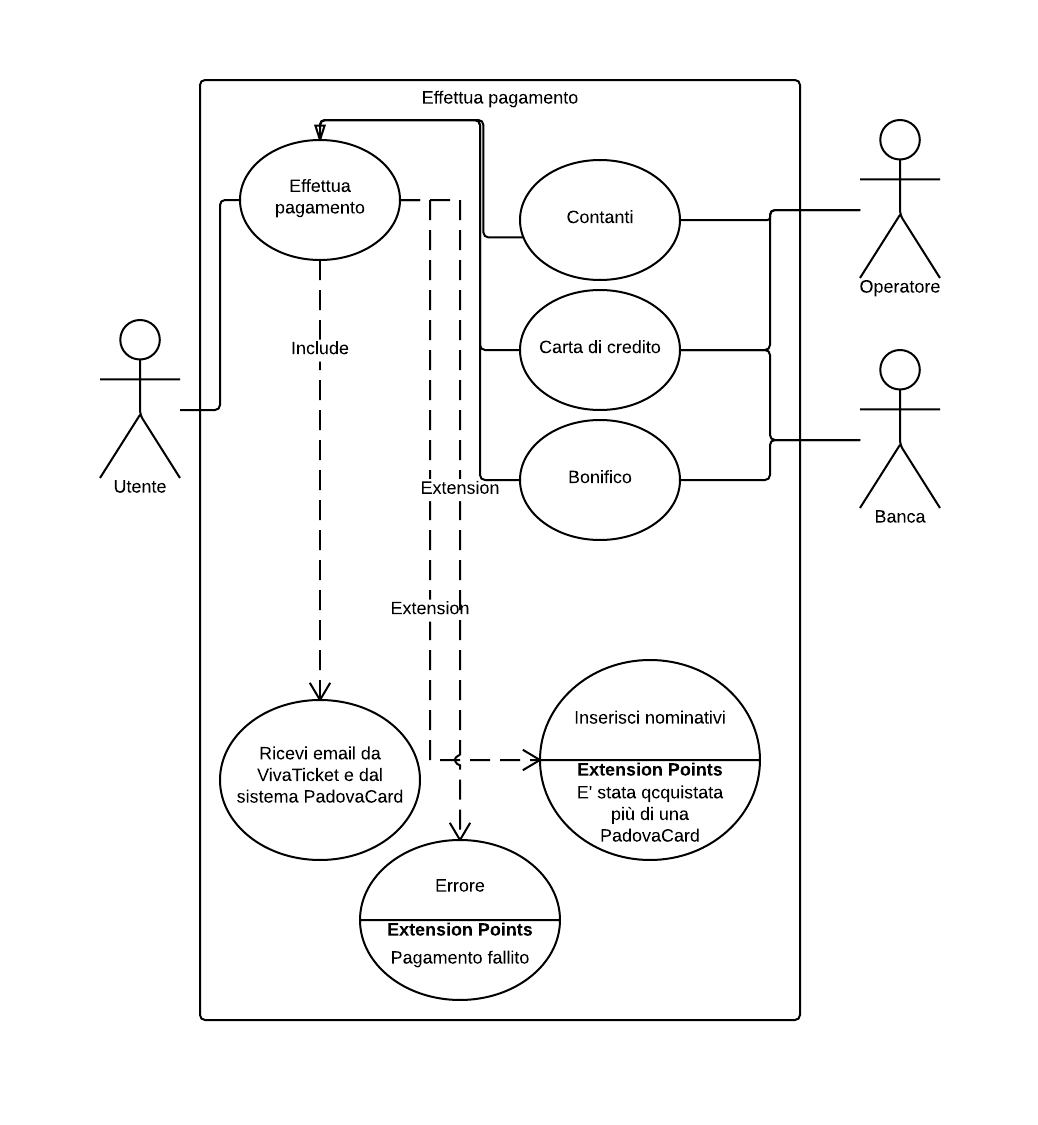
\includegraphics[width=1\textwidth]{images/UCF2.png}
\caption{Caso d'uso UCF2: Acquisto via internet}
\end{figure}
\begin{itemize}
\item \textbf{Attori:} Utente, \charta;
\item \textbf{Descrizione:} L'utente si collega alla piattaforma \vivaticket, direttamente o reinderizzato dal portale descritto in \ref{UC1}. Come già ora accade esso completerà l'operazione su \vivaticket. L'ultima operazione per poter ricevere le PadovaCard è il pagamento, descritto in \ref{UC6}.
\item \textbf{Precondizione:} L'utente desidera comprare una o più padova card;
\item \textbf{Flusso principale degli eventi:}
	\begin{itemize}
		\item L'utente si collega a \vivaticket;
		\item L'utente seleziona il pacchetto desiderato.
	\end{itemize}
\item \textbf{Postcondizione:} L'utente deve solamente pagare per completare l'acquisto.
\end{itemize}

\subsubsection{Caso d'uso UCF3: Inserisci nominativi}\label{UCF3}

\begin{figure}[H]
\centering
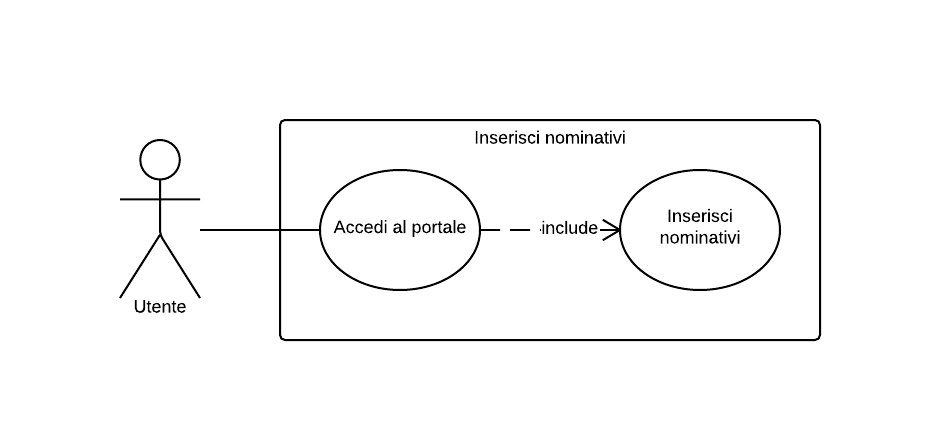
\includegraphics[width=1\textwidth]{images/UCF3.png}
\caption{Caso d'uso UCF3: Inserisci nominativi}
\end{figure}
\begin{itemize}
\item \textbf{Attori:} Utente;
\item \textbf{Descrizione:} Di fronte ad un ordine di più PadovaCard si pone il problema dei nominativi ad esse correlati, come descritto in UC6 - Pagamento (Sezione \ref{UC6}). Per ovviare al problema nel caso in cui l'utente abbia effettuato l'ordine via internet è possibile rendere disponibile una funzionalità che permette all'utente stesso di inserire i nominativi, accedendo al sistema con il codice dell'ordine effettuato su \vivaticket e compilando i form che gli vengono presentati.
\item \textbf{Precondizione:} L'utente è in possesso di più PadovaCard;
\item \textbf{Postcondizione:}  L'utente ha collegato un nominativo per ogni PadovaCard in suo possesso.
\end{itemize}

\subsubsection{Caso d'uso UCF4: Modifica nominativi}
Non è presente un diagramma UML in quanto si tratta di un caso d'uso semplicissimo.
\begin{itemize}
\item \textbf{Attori:} Operatore;
\item \textbf{Descrizione:} Assumendo che l'utente abbia inserito i nominativi, come descritto in UCF3, Sezione \ref{UCF3}, deve essere possibile modificarli, in caso di errore. Se si da tale possibilità all'utente c'è il rischio che ne approfitti per associare diversi proprietari ad un unica PadovaCard, anche se non contemporaneamente. 
L'utente che vuole modificare tali nominativi dovrà quindi contattare un operatore e richiedere la modifica.
\item \textbf{Precondizione:} L'utente ha inserito i nominativi per ogni Padovacard del suo ordine;
\item \textbf{Postcondizione:} L'operatore ha modificato uno o più nominativi.
\end{itemize}

\subsubsection{Caso d'uso UCF6: Creazione utente}
\begin{figure}[H]
\centering
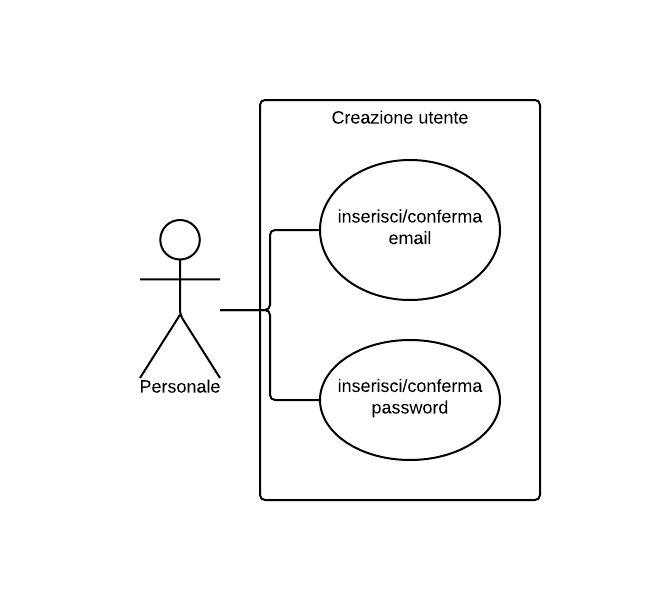
\includegraphics[width=1\textwidth]{images/UCF6.png}
\caption{Caso d'uso UCF6: Creazione utente}
\end{figure}

\begin{itemize}
\item \textbf{Attori:} Personale;
\item \textbf{Descrizione:} Il personale delle strutture deve poter creare il proprio account su OSS;
\item \textbf{Precondizione:} Il membro del personale non possiede un account su OSS;
\item \textbf{Postcondizione:} Il membro del personale possiede un account su OSS.
\end{itemize}

\subsection{Requisiti}
Ogni requisito è identificato da un codice, che segue il seguente formalismo:

\begin{center}
\textbf{R\{X\}\{Y\} \{Gerarchia\}}
\end{center}

Dove:
\begin{itemize}
\item X corrisponde alla priorità del requisito e può assumere i seguenti valori:
	\begin{itemize}
		\item O = Obbligatorio;
        \item F = Facoltativo o opzionale.
	\end{itemize}
\item Y corrisponde al sistema di riferimento e può assumere i seguenti valori:
	\begin{itemize}
		\item O = Operatore, si tratta di operatori degli sportelli IAT o del call center;
        \item U = Utente, si tratta del fruitore della PadovaCard, tipicamente un turista;
        \item P = Personale, si tratta del personale dei luoghi d'interesse convenzionati con PadovaCard;
        \item S = Sistema, si tratta del sistema che si occupa della gestione della PadovaCard.
	\end{itemize}
\item Gerarchia identifica la relazione gerarchica che c'è tra i requisiti di uno stesso tipo. C'è quindi una struttura gerarchica per ogni tipologia di requisito.
\end{itemize}

\newpage

\def\arraystretch{2}
\begin{center}
\begin{longtable}[H]{| p{.20\textwidth} | p{.60\textwidth} | p{.20\textwidth}|}
\hline 
Requisito & Descrizione & Fonti \\ \hline
ROU 1 & L'utente deve poter consultare online le offerte relative alla propria padova card  & UC1 \\ \hline
ROU 2 & L'utente, tramite operatore deve poter comunicare i nominativi associati ad ogni tessera, se su \tlite ne è stata acquistata più di una all'interno di un solo ordine. & UC6 \\ \hline
ROU 3 & L'utente può acquistare uno degli n pacchetti preconfigurati chiamando il call center, pagando con carta di credito o bonifico e ricevere via mail il codice. & UC3, UC6 \\ \hline
ROU 4 & L'utente può acquistare uno degli n pacchetti preconfigurati in uno degli alberghi convenzionati pagando con carta di credito o bonifico e riceve via mail il codice, e opzionalmente un \glossario{voucher} cartaceo. & UC5, UC6 \\ \hline
ROU 5 & L'utente può acquistare uno degli n pacchetti preconfigurati, o comporre il proprio ad uno sportello IAT, pagando con carta di credito o contanti e riceverà la tessera ed eventualmente il codice via mail.  & UC4, UC6 \\ \hline
ROU 6 & L'utente può accedere alla struttura solo se è prevista all'interno della sua PadovaCard, se essa non è scaduta (superato il periodo di validità) e se non ha già effettuato la visita.  & UC8 \\ \hline
ROU 7 & L'utente può farsi stampare una nuova tessera in caso essa venga smarrita. (L'utente è comunque in possesso del codice su email).  & UC7 \\ \hline
RFU 8 & L'utente deve inserire autonomamente la data e l'ora di inizio validità della PadovaCard.  & UC6 \\ \hline
RFU 9 & L'utente può acquistare uno degli n pacchetti preconfigurati su \vivaticket pagando con carta di credito e ricevere via mail il codice. & UCF2, UC6 \\ \hline
RFU 10 & L'utente può comporre la propria PadovaCard, visualizzando in tempo reale prezzi ed offerte dei vari pacchetti/ingressi.  & UCF1.1, UCF1.2, UCF1.3 \\ \hline
RFU 11 & L'utente può stampare un codice relativo alla propria composizione ed acquistarla ad uno sportllo IAT.  & UCF1.2, UCF1.3 \\ \hline
RFU 13 & L'utente, tramite il portale deve poter inserire i nominativi associati ad ogni tessera, se su vivaticket ne è stata acquistata più di una all'interno di un solo ordine.  & UCF3 \\ \hline
ROP 14 & Il personale deve loggarsi al sistema con un id univoca.  & UC9 \\ \hline
ROP 15 & Il personale deve poter recuperare la propria password in caso di smarrimento.  & UC9 \\ \hline
ROP 16 & Il personale deve poter modificare la propria password.  & UC9 \\ \hline
ROP 17 & Il personale avrà un lettore di codici che rileverà il codice presente sulla tessera, sul \glossario{voucher} o a a schermo, nel caso in cui l'utente utilizzi la mail su cellulare.  & UC8 \\ \hline
RFP 18 & Il personale deve poter creare un account su OSS & UCF6 \\ \hline
ROO 19 & Gli operatori devono loggarsi al sistema con un id univoca.  & UC9 \\ \hline
ROO 20 & Gli operatori devono poter recuperare la propria password in caso di smarrimento.  & UC9 \\ \hline
ROO 21 & Gli operatori devono poter modificare la propria password.  & UC9 \\ \hline
ROO 22 & Gli operatori potranno selezionare su \tlite un biglietto di costo zero.  & UC4, UC3 \\ \hline
ROO 23 & L'operatore dovrà poter inserire nel sistema i nominativi associati alle padovacard se queste sono state acquistate su \tlite tramite un unico ordine.  & UC6 \\ \hline
ROO 24 & Gli operatori IAT effettuano un unico pagamento nel caso in cui vengano combinati l'acquisto di una o più padova card sia con i pacchetti predefiniti sia personalizzate e altri articoli in vendita (mappe, guide, souvenir etc.). & UC6 \\ \hline
ROO 25 & Gli operatori possono modificare, su richiesta dell'utente il periodo di validità di una Padovacard già acquistata. & UC2 \\ \hline
ROS 26 & Il sistema partendo dai dati ricevuti da \tlite genererà un codice univoco per ogni tessera e vi associerà tutte le informazioni, per poi salvarle nel database.  &  \\ \hline
ROS 27 & Allo scadere del periodo di validità il sistema marca il codice della carta come non più valida. &  \\ \hline
ROS 28 & Quando si effettua una visita il sistema marca tale visita non più effettuabile da parte di quel codice.  &  \\ \hline
ROS 29 & Il sistema mantiene separati i dati relativi alle PadovaCard da tutti gli altri, ma raggruppa i dati sulle vendite, per cui la vendita di una PadovaCard è salvata assieme a qualunque altra vendita, ma nessuna informazione è fornita su tale padovaCard se non il codice.  &  \\ \hline
RFS 31 & Il sistema riconosce come non valida una tessera a cui non è associato un nominativo. &  \\ \hline
RFO 31 & Gli operatori devono poter modificare i nominativi di un ordine già pagato. & UCF4 \\ \hline
\caption{Tabella requisiti}
\end{longtable}
\end{center}


%\section{Glossario}
\definizione{CakePhp}: framework per la realizzazione di applicazioni web scritto in PHP. È ispirato al concetto di \glossario{MVC}. \\
\definizione{IAT} Acronimo di Informazioni assistenza turistica, si tratta degli uffici o sportelli sparsi per la città in cui si possono ottenere informazioni, e acquistare/ricevere la PadovaCard. \\
\definizione{MVC}: Acronimo di Model View Controller, è un Design Pattern architetturale che divide l’applicazione in tre parti interconnesse, separando l’interfaccia utente, la logica e i dati. \\
\definizione{Operatore}: si tratta di operatori degli sportelli \glossario{IAT} o del call center;\\
\definizione{OSS}:  \\
\definizione{Personale}: si tratta del personale delle \glossario{strutture} convenzionate con PadovaCard, si occuperanno di verificarne la validità. \\
\definizione{Struttura}: si fa riferimento alle strutture convenzionate con PadovaCard, e quindi visitabili dagli \glossario{utenti} che ne sono in possesso \\
\definizione{Utente}: si tratta del fruitore della PadovaCard, tipicamente un turista.\\
\definizione{Voucher}: documenti emessi da agenzie di viaggio ai propri clienti, come conferma del diritto a godere, nel loro viaggio, di specifici servizi, in essi indicati e già pagati in precedenza all'agenzia stessa. In questo caso si tratta di un foglio formato A4 stampato dall'hotel che ha il valore di una PadovaCard in quanto su di esso è riportato il codice a barre relativo. \\
  


\end{document}